\documentclass[11pt,a4paper]{article}

\usepackage[T1]{fontenc}
\usepackage[utf8]{inputenc}
\usepackage[sc]{mathpazo}
\linespread{1.06}
\usepackage{amsmath,amssymb,mathtools}
\usepackage[a4paper,margin=2.6cm,headheight=14pt]{geometry}
\usepackage{tikz}
\usetikzlibrary{arrows.meta,positioning,decorations.pathmorphing,calc}
\usepackage[most]{tcolorbox}
\usepackage{enumitem}
\usepackage{booktabs}
\usepackage{microtype}
\usepackage{fancyhdr}

% ---------- cores (antes do hyperref) ----------
\definecolor{azulesc}{HTML}{1F3864}
\definecolor{azulclaro}{HTML}{E8EEF7}
\definecolor{vermelhoesc}{HTML}{8B2500}
\definecolor{vermelhoclaro}{HTML}{FBEAE3}
\definecolor{verdeesc}{HTML}{1F5C3A}
\definecolor{verdeclaro}{HTML}{E6F2EA}
\definecolor{cinza}{HTML}{5A5A5A}
\definecolor{ocre}{HTML}{B8860B}

\usepackage[colorlinks=true,linkcolor=azulesc,citecolor=azulesc,urlcolor=azulesc]{hyperref}

% ---------- cabecalho ----------
\pagestyle{fancy}
\fancyhf{}
\fancyhead[L]{\small\color{cinza}Do zero ao trímero — Parte II}
\fancyhead[R]{\small\color{cinza}\thepage}
\renewcommand{\headrulewidth}{0.4pt}

% ---------- caixas ----------
\newtcolorbox{suavez}[1][]{
  enhanced, breakable,
  colback=vermelhoclaro, colframe=vermelhoesc,
  boxrule=0.9pt, arc=2pt, left=10pt,right=10pt,top=8pt,bottom=8pt,
  fonttitle=\bfseries\sffamily,
  title={Sua vez\ #1}}

\newtcolorbox{atencao}[1][]{
  enhanced, breakable,
  colback=white, colframe=ocre,
  boxrule=0.9pt, arc=2pt, left=10pt,right=10pt,top=8pt,bottom=8pt,
  fonttitle=\bfseries\sffamily,
  title={#1}}

\newtcolorbox{ideia}[1][]{
  enhanced, breakable,
  colback=azulclaro, colframe=azulesc,
  boxrule=0.9pt, arc=2pt, left=10pt,right=10pt,top=8pt,bottom=8pt,
  fonttitle=\bfseries\sffamily,
  title={#1}}

\newtcolorbox{ponte}[1][]{
  enhanced, breakable,
  colback=verdeclaro, colframe=verdeesc,
  boxrule=0.9pt, arc=2pt, left=10pt,right=10pt,top=8pt,bottom=8pt,
  fonttitle=\bfseries\sffamily,
  title={#1}}

% ---------- atalhos ----------
\newcommand{\hbtm}{\frac{\hbar^{2}}{2m_{r}}}
\newcommand{\dd}{\mathrm{d}}
\renewcommand{\vec}[1]{\mathbf{#1}}
\newcommand{\bxi}{\vec{\xi}}

\setlength{\parskip}{0.35em}

\title{\vspace{-1.5cm}\Huge\bfseries Do zero ao trímero\\[0.25cm]
\LARGE\mdseries Parte II — unitariedade, o hiper-raio e a torre}
\author{\large Notas de estudo · Pedro Henrique G. Modesto\\[0.15cm]
\normalsize Mestrado IFSC/USP · orientação: Lucas Madeira}
\date{\normalsize Agosto de 2026}

\begin{document}
\maketitle
\thispagestyle{empty}

\begin{ideia}[Como usar este texto]
Igual à Parte I, com uma diferença: aqui há \textbf{onze} caixas vermelhas
\textbf{Sua vez}, não quatro. Você pediu para ser mais ativo, e a matéria desta parte
permite — quase toda conta daqui é curta, e quase toda tem um final que vale a pena.

Faça-as com caneta, sem consultar o resto do texto. As de número \textbf{6} e
\textbf{9} são as duas que sustentam a dissertação inteira; se você só fizer duas,
faça essas.

Ao lado de várias seções há uma caixa verde \textbf{No computador}, apontando a
estação do notebook unificado onde aquilo vira código rodando. A ideia é: fecha a
conta no papel, roda a estação, vê o mesmo número aparecer.
\end{ideia}

\vspace{0.3cm}

\section*{Onde estamos indo}
\addcontentsline{toc}{section}{Onde estamos indo}

Na Parte I você fechou os três primeiros degraus. Esta parte fecha o quarto e o
quinto — e o quinto é o degrau que a dissertação inteira pisa.

\begin{center}
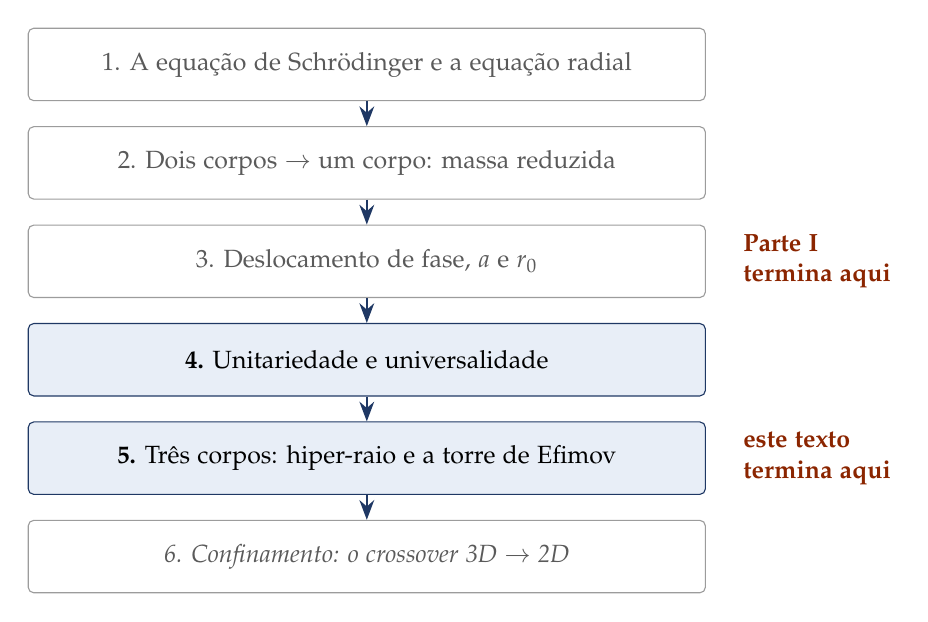
\begin{tikzpicture}[
  feito/.style={draw=cinza!60, fill=white, rounded corners=2pt,
                minimum width=8.6cm, minimum height=0.92cm, align=center,
                font=\small, text=cinza},
  degrau/.style={draw=azulesc, fill=azulclaro, rounded corners=2pt,
                 minimum width=8.6cm, minimum height=0.92cm, align=center,
                 font=\small},
  futuro/.style={draw=cinza!60, fill=white, rounded corners=2pt,
                 minimum width=8.6cm, minimum height=0.92cm, align=center,
                 font=\small\itshape, text=cinza},
  seta/.style={-{Stealth[length=2.5mm]}, azulesc, thick}
]
\node[feito]  (d1) at (0,0)     {1. A equação de Schrödinger e a equação radial};
\node[feito]  (d2) at (0,-1.25) {2. Dois corpos $\to$ um corpo: massa reduzida};
\node[feito]  (d3) at (0,-2.5)  {3. Deslocamento de fase, $a$ e $r_{0}$};
\node[degrau] (d4) at (0,-3.75) {\textbf{4.} Unitariedade e universalidade};
\node[degrau] (d5) at (0,-5.0)  {\textbf{5.} Três corpos: hiper-raio e a torre de Efimov};
\node[futuro] (d6) at (0,-6.25) {6. Confinamento: o crossover 3D $\to$ 2D};
\draw[seta] (d1) -- (d2);
\draw[seta] (d2) -- (d3);
\draw[seta] (d3) -- (d4);
\draw[seta] (d4) -- (d5);
\draw[seta] (d5) -- (d6);
\node[right=0.35cm of d3, font=\small\bfseries, text=vermelhoesc, align=left]
  {Parte I\\termina aqui};
\node[right=0.35cm of d5, font=\small\bfseries, text=vermelhoesc, align=left]
  {este texto\\termina aqui};
\end{tikzpicture}
\end{center}

Uma frase para orientar a leitura: \emph{tudo nesta parte é consequência de uma
simetria e da maneira estranha como ela se quebra.} Se em algum momento a conta
parecer arbitrária, volte a essa frase — ela é o fio.

% =====================================================================
\section{Unitariedade e universalidade}
\label{sec:unit}
% =====================================================================

\subsection{O que ``esquecer o potencial'' quer dizer}

A expansão de alcance efetivo da Parte I,
\begin{equation}
k\cot\delta_{0}(k) = -\frac{1}{a} + \frac{1}{2}r_{0}k^{2} + \mathcal{O}(k^{4}),
\label{eq:ere}
\end{equation}
diz que a baixa energia o potencial inteiro comparece por dois números. Agora
pergunte: e se um deles for muito maior que o outro?

Quando $|a| \gg r_{0}$, o termo $\tfrac12 r_{0}k^{2}$ é desprezível em toda a região
onde $k|a|\lesssim 1$. Sobra
\begin{equation}
k\cot\delta_{0}\simeq -\frac{1}{a},
\qquad\text{e a seção de choque}\qquad
\sigma = \frac{4\pi}{k^{2}+1/a^{2}}.
\end{equation}
Nenhuma outra propriedade do potencial aparece. Dois potenciais completamente
diferentes com o mesmo $a$ dão a \emph{mesma} física. Isso é a
\textbf{universalidade}, e ela não é uma aproximação de conveniência: é uma
consequência de $\lambda_{\text{dB}} \gg$ alcance.

O caso extremo, $1/a \to 0$, chama-se \textbf{unitariedade}. Ali
$\sigma = 4\pi/k^{2}$: a seção de choque satura o máximo permitido pela
conservação de probabilidade em onda-$s$ — daí o nome.

\begin{atencao}[Um erro que quase todo mundo comete uma vez]
$a \to \infty$ \emph{não} significa interação infinitamente forte, nem alcance
infinito. O potencial continua curto e finito. O que diverge é o
\emph{comprimento de espalhamento} --- uma propriedade da solução, não do potencial.
Foi exatamente isso que você viu no poço em $K_{0}R = \pi/2$: profundidade finita,
alcance finito, $a$ infinito.
\end{atencao}

\subsection{Escala: a simetria que aparece na unitariedade}

Aqui está o ponto que a Parte I prometeu e não entregou. Na unitariedade, a energia
zero e fora do alcance, a equação radial é apenas
\begin{equation}
u''(r) = 0.
\end{equation}
Não há nenhum comprimento nela. E um problema sem comprimento característico não
consegue distinguir ``perto'' de ``longe'': ele é \textbf{invariante por mudança de
escala}.

\begin{suavez}[\;1 — a simetria de escala, e quem a quebra]
Faça a mudança $r \to \lambda r$ (com $\lambda>0$ constante) e mostre que:
\begin{enumerate}[label=(\alph*), itemsep=2pt]
\item a equação $u''=0$ é invariante;
\item a condição de contorno $u'(0)/u(0) = -1/a$ \emph{não} é --- ela vira
      $-1/(\lambda a)$.
\end{enumerate}
Conclua em uma frase: quem quebra a invariância de escala do problema de dois corpos?
E o que acontece com essa quebra quando $a\to\infty$?

\vspace{2.2cm}
\hrulefill
\end{suavez}

O que você acabou de mostrar é a espinha desta parte inteira: \textbf{$a$ é a única
escala do problema de dois corpos}, e na unitariedade ela some. O sistema fica
invariante por escala contínua.

Guarde essa frase com carinho. Em três corpos ela vai ser \emph{quase} verdadeira, e
a palavra ``quase'' é o efeito Efimov.

\begin{ponte}[No computador — Estação 6]
A estação de unitariedade varre $v$ no poço esférico e mostra $1/a$ cruzando o zero.
Repare que o \emph{gráfico} de $1/a$ é liso e sem drama; é $a$ que explode. Perseguir
$1/a$ em vez de $a$ é a escolha certa em todo o resto do mestrado.
\end{ponte}

\subsection{O pseudopotencial: jogar o potencial fora de vez}

Se a baixa energia só $a$ importa, por que carregar $V(r)$? Não precisa. Substitua o
potencial inteiro por uma \textbf{condição de contorno} na origem.

Fora do alcance e a energia zero, $u = C(r-a)$. Então:

\begin{suavez}[\;2 — a condição de Bethe--Peierls]
Calcule $u'(r)/u(r)$ para $u = C(r-a)$ e tome $r\to 0$ (mais precisamente:
$r$ maior que o alcance, mas muito menor que $|a|$ e que $1/k$). Mostre que
\[
\frac{u'}{u}\bigg|_{r\to 0} = -\frac{1}{a}
\qquad\Longleftrightarrow\qquad
\frac{(r\psi)'}{r\psi}\bigg|_{r\to 0} = -\frac{1}{a}.
\]
Uma linha. Depois responda: por que essa condição carrega \emph{exatamente} a mesma
informação física que o potencial inteiro, no regime de baixa energia?

\vspace{2.0cm}
\hrulefill
\end{suavez}

Essa é a \textbf{condição de Bethe--Peierls}, e é o modelo de alcance zero completo:
sem potencial, um número. Toda a física de Efimov que vem a seguir é construída em
cima dela --- inclusive o \texttt{efimov.py} do seu repositório.

\begin{atencao}[O preço, explicitamente]
Alcance zero implica $r_{0}=0$. Você joga fora, de propósito:
os estados ligados profundos, tudo em $k \gtrsim 1/r_{0}$, e a estrutura da função de
onda dentro do alcance. Fica só o estado raso e a física universal.

É um preço alto e é pago com prazer, porque em troca a teoria vale para
$^{39}$K, $^{133}$Cs, $^{4}$He e para o dêuteron, com a \emph{mesma} equação. E é
por isso que o alcance efetivo é interessante: ele é a primeira correção a esse
preço --- o assunto do Madeira (2024), e o motivo pelo qual o Lucas te mandou
reproduzir o artigo de alcance efetivo antes de qualquer outra coisa.
\end{atencao}

\subsection{O dímero raso}

Com $a>0$ há um estado ligado, e ele é raso: sua energia deve ser construída só com
$\hbar$, $m_{r}$ e $a$. Por análise dimensional, só há uma combinação possível.

\begin{suavez}[\;3 — a energia do dímero, e a primeira correção]
\textbf{(a)} Procure solução ligada $u \propto e^{-\kappa r}$ fora do alcance, imponha
a condição de Bethe--Peierls da \textbf{Sua vez 2} e mostre que $\kappa = 1/a$, logo
\[
E_{\text{zr}} = -\frac{\hbar^{2}}{2m_{r}a^{2}}.
\]
\textbf{(b)} Agora não jogue $r_{0}$ fora. Em \eqref{eq:ere}, o estado ligado
corresponde ao polo em $k = i\kappa$, isto é, $k\cot\delta_{0} \to -\kappa$.
Substitua e mostre que
\[
\frac{1}{a} = \kappa - \frac{1}{2}r_{0}\kappa^{2}.
\]
Resolva para $\kappa$ (raiz física: a que tende a $1/a$ quando $r_{0}\to 0$).

\vspace{2.6cm}
\hrulefill
\end{suavez}

O item (b) é a Eq.~(95) do artigo, e é o que o \texttt{analitico.py} chama de
\texttt{energia\_fr}. Você acabou de derivar uma função que já rodou centenas de vezes
na sua máquina.

\begin{ponte}[No computador — Estação 5]
A estação do dêuteron compara $E_{\text{zr}}$ e $E_{\text{fr}}$ com o valor
experimental. A diferença entre as duas colunas é, literalmente, o tamanho do preço
que você acabou de calcular em (b).
\end{ponte}

% =====================================================================
\section{Três corpos: montando o palco}
\label{sec:tres}
% =====================================================================

\subsection{O problema, e por que ele não é ``dois corpos de novo''}

Três partículas em 3D têm nove coordenadas. Tirando o centro de massa, sobram seis.
Não há como reduzir mais: seis é o número irredutível.

E aqui morre a esperança de repetir a Parte I. Com dois corpos, o vetor relativo
$\vec r$ tinha um módulo e uma direção, e a simetria esférica separava
$r$ de $(\theta,\varphi)$ perfeitamente. Com seis coordenadas você ainda pode separar
\emph{um} módulo de \emph{cinco} ângulos --- mas os cinco ângulos agora carregam
física de verdade, porque descrevem a \emph{forma} do triângulo, e a interação
depende dela.

A estratégia é a mesma de sempre, e é o que dá certo:
\begin{center}
\fbox{\parbox{0.86\textwidth}{\centering
separar \textbf{tamanho} de \textbf{forma}, resolver a forma primeiro, e deixar o
tamanho com uma equação radial de uma variável só.}}
\end{center}

\subsection{Coordenadas de Jacobi}

Para três massas iguais $m$, defina
\begin{equation}
\bxi_{1} = \frac{\vec r_{1}-\vec r_{2}}{\sqrt{2}},
\qquad
\bxi_{2} = \frac{\vec r_{1}+\vec r_{2}-2\vec r_{3}}{\sqrt{6}},
\qquad
\vec R_{\text{cm}} = \frac{\vec r_{1}+\vec r_{2}+\vec r_{3}}{3}.
\label{eq:jacobi}
\end{equation}
O $\bxi_{1}$ é ``onde está a partícula 1 em relação à 2''; o $\bxi_{2}$ é ``onde está
a 3 em relação ao par''. Os fatores $\sqrt2$ e $\sqrt6$ parecem gratuitos. Não são:
são exatamente o que faz a energia cinética ficar bonita.

\begin{suavez}[\;4 — por que esses fatores, e não outros]
Mostre que, com \eqref{eq:jacobi},
\[
\sum_{i} \frac{\vec p_{i}^{\,2}}{2m}
= \frac{\vec P_{\text{cm}}^{\,2}}{2(3m)}
+ \frac{\vec p_{\xi_{1}}^{\,2}}{2m} + \frac{\vec p_{\xi_{2}}^{\,2}}{2m}.
\]
Ou seja: sem termos cruzados, e com a \emph{mesma} massa $m$ nas duas partes.

\emph{Atalho, se preferir:} basta verificar a identidade equivalente para as
velocidades, $\sum_i \dot{\vec r}_i^{\,2} = 3\dot{\vec R}_{\text{cm}}^{\,2}
+ \dot{\bxi}_{1}^{\,2} + \dot{\bxi}_{2}^{\,2}$, que é álgebra pura.

\vspace{2.4cm}
\hrulefill
\end{suavez}

Esse é o milagre técnico das coordenadas de Jacobi com massa escalada: as duas
direções relativas entram com \textbf{a mesma massa}, então o operador cinético é um
único laplaciano num espaço de $3+3=6$ dimensões:
\begin{equation}
\hat T_{\text{rel}} = -\frac{\hbar^{2}}{2m}\left(\nabla^{2}_{\xi_{1}} +
\nabla^{2}_{\xi_{2}}\right)
= -\frac{\hbar^{2}}{2m}\,\nabla^{2}_{(6)}.
\label{eq:T6}
\end{equation}

\begin{ideia}[A frase que faz tudo funcionar]
Três partículas em 3D $\equiv$ \textbf{uma} partícula em 6D.

Não é analogia: é igualdade. Toda a maquinaria da Parte I --- equação radial,
substituição $u=rR$, barreira centrífuga --- vai valer aqui sem mudar uma vírgula.
Só o número de dimensões muda.
\end{ideia}

\subsection{O hiper-raio: o tamanho do triângulo}

Defina
\begin{equation}
\rho^{2} = \xi_{1}^{2} + \xi_{2}^{2}.
\end{equation}
É simplesmente o ``raio'' do vetor de seis componentes. Mas ele tem um significado
geométrico muito mais bonito do que parece.

\begin{suavez}[\;5 — o hiper-raio é o tamanho do triângulo]
Mostre que, com \eqref{eq:jacobi},
\[
\rho^{2} = \frac{1}{3}\left(r_{12}^{2} + r_{23}^{2} + r_{31}^{2}\right),
\qquad r_{ij} \equiv |\vec r_{i}-\vec r_{j}|.
\]
\emph{Sugestão:} expanda os dois lados em termos de $\vec r_i \cdot \vec r_j$, ou
teste com o caso particular $\vec r_1 = (1,0,0)$, $\vec r_2 = \vec r_3 = \vec 0$ e
depois generalize.

Em seguida responda: se você dobrar o triângulo de tamanho \emph{sem mudar a forma},
o que acontece com $\rho$? E se você deformar a forma mantendo $\rho$ fixo?

\vspace{2.4cm}
\hrulefill
\end{suavez}

Pronto: $\rho$ mede o tamanho global do trio, democraticamente --- os três pares
entram com o mesmo peso. Os cinco ângulos restantes (os \emph{hiper-ângulos})
descrevem a forma: se o triângulo é equilátero, alongado, se dois átomos estão
grudados e o terceiro longe. Chame-os coletivamente de $\Omega$.

\begin{atencao}[O que $\rho\to 0$ e $\rho\to\infty$ significam]
$\rho\to 0$: os três átomos juntos no mesmo ponto. $\rho\to\infty$: o trio grande ---
mas isso inclui tanto ``três átomos separados'' quanto ``um dímero pequeno e o
terceiro átomo muito longe''. Distinguir esses dois casos é papel dos \emph{ângulos},
não de $\rho$. Guarde: é daí que sai o contínuo partícula-dímero da Fig.~1 do seu
projeto.
\end{atencao}

% =====================================================================
\section{A equação radial em \texorpdfstring{$d$}{d} dimensões}
\label{sec:radial}
% =====================================================================

Agora vem o degrau que a Parte I prometeu: de onde sai o $\tfrac14$.

O laplaciano em $d$ dimensões, separado em raio e ângulos, é
\begin{equation}
\nabla^{2}_{(d)} = \frac{\partial^{2}}{\partial\rho^{2}}
+ \frac{d-1}{\rho}\frac{\partial}{\partial\rho}
+ \frac{1}{\rho^{2}}\Lambda^{2}_{(d)},
\label{eq:lapd}
\end{equation}
onde $\Lambda^{2}_{(d)}$ é o operador angular generalizado, cujos autovalores são
$-\lambda(\lambda+d-2)$. (Para $d=3$ isso é o $-\ell(\ell+1)$ de sempre; confira.)

O termo $\frac{d-1}{\rho}\partial_{\rho}$ é o \textbf{jacobiano} disfarçado: em $d$
dimensões, a casca esférica de raio $\rho$ tem área $\propto \rho^{d-1}$. É ele que
vai produzir o $\tfrac14$ --- e é por isso que o $\tfrac14$ não é física de Efimov, é
geometria.

Separe $\Psi = \psi(\rho)\,Y_{\lambda}(\Omega)$ e elimine a primeira derivada com a
substituição generalizada do $u=rR$ da Parte I:
\begin{equation}
\boxed{\;\psi(\rho) = \rho^{-\frac{d-1}{2}}\,u(\rho).\;}
\label{eq:sub}
\end{equation}

\begin{suavez}[\;6 — a conta que sustenta a dissertação]
Substitua \eqref{eq:sub} em \eqref{eq:lapd} e mostre que a equação radial fica
\[
u''(\rho) + \left[\,k^{2} - U(\rho) - \frac{L^{2}-\tfrac14}{\rho^{2}}\,\right]u(\rho) = 0,
\qquad
\boxed{L = \lambda + \frac{d-2}{2}}.
\]
\emph{Roteiro (não é difícil, é só organizado):}
\begin{enumerate}[label=\arabic*., itemsep=2pt, leftmargin=*]
\item Calcule $\psi'$ e $\psi''$ pela regra do produto.
\item Monte $\psi'' + \frac{d-1}{\rho}\psi'$ e verifique que os termos em $u'$ se
      cancelam --- é para isso que serve o expoente $-\tfrac{d-1}{2}$.
\item Sobra um termo em $u/\rho^{2}$ com coeficiente $\frac{(d-1)(3-d)}{4}$.
      Some com $-\lambda(\lambda+d-2)$.
\item Complete o quadrado: mostre que
      $\lambda(\lambda+d-2) = L^{2} - \frac{(d-2)^{2}}{4}$ com $L$ acima, e que os
      pedaços restantes somam exatamente $-\tfrac14$.
\end{enumerate}

\vspace{3.2cm}
\hrulefill
\end{suavez}

\begin{ideia}[O que você acabou de provar]
Uma equação, um parâmetro, três físicas:

\vspace{0.25cm}
\begin{center}
\begin{tabular}{@{}llll@{}}
\toprule
caso & $d$ & $L$ & $L^{2}-\tfrac14$ \\
\midrule
3D, onda parcial $\ell$        & 3 & $\ell+\tfrac12$ & $\ell(\ell+1)$ \\
2D, momento angular $m$        & 2 & $m$             & $m^{2}-\tfrac14$ \\
\textbf{3 corpos, hiper-raio}  & \textbf{6} & \textbf{$s$} & \textbf{$s^{2}-\tfrac14$} \\
\bottomrule
\end{tabular}
\end{center}
\vspace{0.25cm}

A primeira linha é a Parte I. A terceira é o resto deste texto. E a segunda é o
destino do seu mestrado --- porque $d$ aparece \textbf{como um parâmetro contínuo},
e girá-lo de 3 até 2 é exatamente o crossover dimensional.

O $\tfrac14$ é o jacobiano em seis dimensões. Não tem nada a ver com Efimov.
\end{ideia}

\begin{suavez}[\;7 — o teste de sanidade]
Confira que sua fórmula reproduz o que você já sabe: ponha $d=3$ e $\lambda=\ell$ e
verifique que $L^{2}-\tfrac14 = \ell(\ell+1)$. Depois ponha $d=3$, $\ell=0$ e confirme
que o termo some inteiro --- como tinha que ser na Parte I.

\vspace{1.6cm}
\hrulefill
\end{suavez}

\begin{ponte}[No computador — Estação 7]
A estação do solver unificado tem exatamente esse parâmetro. Você passa $d$ e
$\lambda$, e o mesmo integrador da Estação 2 resolve onda-$p$, 2D e Efimov. É a
tradução direta da sua Sua vez 6 --- e é o Eixo 1 do plano do repositório.
\end{ponte}

% =====================================================================
\section{O canal hiperangular e o número \texorpdfstring{$s_{0}$}{s0}}
% =====================================================================

Falta saber quanto vale $L$ no caso de três corpos. Em dois corpos, $\ell$ era um
inteiro porque a função de onda tinha que ser univalorada ao dar a volta. Aqui não é
tão simples: a equação angular sente a interação, através da condição de
Bethe--Peierls imposta quando \emph{dois} dos três átomos se encontram.

O resultado (Efimov, 1970; Danilov, 1961) é que, para três bósons idênticos na
unitariedade, o autovalor angular $s$ não é inteiro: ele resolve
\begin{equation}
\boxed{\;s\cos\!\left(\frac{\pi s}{2}\right)
= \frac{8}{\sqrt3}\,\sin\!\left(\frac{\pi s}{6}\right).\;}
\label{eq:transc}
\end{equation}
Essa equação não tem raiz real pequena. Ela tem raiz \textbf{imaginária}.

\begin{suavez}[\;8 — a raiz imaginária]
Ponha $s = i\,s_{0}$ em \eqref{eq:transc}, use
$\cos(ix)=\cosh x$ e $\sin(ix)=i\sinh x$, e mostre que a equação vira
\[
s_{0}\cosh\!\left(\frac{\pi s_{0}}{2}\right)
= \frac{8}{\sqrt3}\,\sinh\!\left(\frac{\pi s_{0}}{6}\right).
\]
Depois \textbf{verifique numericamente} (calculadora serve) que $s_{0}=1{,}00624$
satisfaz: os dois lados devem dar $\approx 2{,}5476$.

\vspace{2.2cm}
\hrulefill
\end{suavez}

Com $s = is_{0}$, o termo centrífugo da Seção~\ref{sec:radial} muda de sinal:
\begin{equation}
L^{2}-\tfrac14 = (is_{0})^{2}-\tfrac14 = -\left(s_{0}^{2}+\tfrac14\right),
\end{equation}
e a equação radial no hiper-raio fica
\begin{equation}
\boxed{\;u''(\rho) + \left[\frac{2mE}{\hbar^{2}}
+ \frac{s_{0}^{2}+\tfrac14}{\rho^{2}}\right]u(\rho)=0.\;}
\label{eq:efimov}
\end{equation}

\begin{atencao}[Pare e repare no que aconteceu]
O termo centrífugo é \textbf{sempre repulsivo} --- é a barreira que impede a
partícula de chegar na origem. Foi assim a Parte I inteira.

Aqui ele virou \textbf{atração}. Três corpos ressonantes produzem uma atração
efetiva de longo alcance que \emph{não existe} em dois corpos. Ela não vem de nenhuma
força de três corpos que alguém colocou na mão: vem da geometria de seis dimensões
mais a condição de contorno de dois corpos.

É esse sinal trocado que é o efeito Efimov.
\end{atencao}

% =====================================================================
\section{A queda ao centro e a torre}
% =====================================================================

\subsection{O potencial \texorpdfstring{$-1/\rho^{2}$}{-1/rho2} é o caso crítico}

Um potencial $\propto 1/\rho^{2}$ é especial porque tem a \emph{mesma} dimensão do
termo cinético. Multiplicar $\rho$ por $\lambda$ multiplica os dois pelo mesmo fator:
ele é invariante por escala. Não há competição entre os dois termos --- e sem
competição, não há um tamanho preferido.

\begin{suavez}[\;9 — a segunda conta que sustenta a dissertação]
Considere $u'' + \dfrac{c}{\rho^{2}}u = 0$ e procure solução de potência,
$u = \rho^{\alpha}$.
\begin{enumerate}[label=(\alph*), itemsep=2pt]
\item Mostre que $\alpha$ satisfaz $\alpha^{2}-\alpha+c = 0$ e resolva.
\item Para que valor de $c$ as duas raízes deixam de ser reais? (Este é o
      \textbf{coeficiente crítico}.)
\item Com $c = s_{0}^{2}+\tfrac14$, mostre que
      $\alpha = \tfrac12 \pm i\,s_{0}$.
\end{enumerate}

\vspace{2.6cm}
\hrulefill
\end{suavez}

O coeficiente crítico é $c=\tfrac14$ --- e é o mesmo $\tfrac14$ do jacobiano, o que
não é coincidência: a barreira centrífuga em $d$ dimensões e a queda ao centro são o
mesmo problema visto de dois lados. Como $s_{0}^{2}+\tfrac14 > \tfrac14$ sempre, o
caso de Efimov está \emph{sempre} do lado supercrítico.

Escrevendo $\rho^{\frac12 \pm i s_{0}} = \sqrt\rho\;e^{\pm i s_{0}\ln\rho}$ e tomando
combinações reais:
\begin{equation}
u(\rho) = \sqrt{\rho}\,\sin\!\left(s_{0}\ln\rho + \varphi\right).
\label{eq:logper}
\end{equation}

\begin{suavez}[\;10 — confira a solução]
Verifique por substituição direta que \eqref{eq:logper} resolve
$u''+(s_{0}^{2}+\tfrac14)u/\rho^{2}=0$.

Depois olhe para ela e responda: quantos nós essa função tem entre $\rho=0$ e
$\rho=\rho_{\max}$? O que acontece com esse número quando $\rho\to 0$?

\vspace{2.2cm}
\hrulefill
\end{suavez}

\subsection{A catástrofe, e o número que a conserta}

O que você acabou de descobrir no item final da Sua vez 10 é uma catástrofe genuína:
a solução oscila \textbf{infinitas vezes} quando $\rho\to0$, porque ela é periódica em
$\ln\rho$ e $\ln\rho \to -\infty$. Infinitos nós significam infinitos estados ligados,
com energias que descem sem fundo. O hamiltoniano não é auto-adjunto; o problema, do
jeito que está, \textbf{não tem solução}.

A cura é obrigatória e tem nome: você precisa impor uma condição em algum
$\rho_{0}$ pequeno,
\begin{equation}
u(\rho) \;\sim\; \sqrt{\rho}\,\sin\!\left(s_{0}\ln\frac{\rho}{\rho_{0}}\right),
\end{equation}
e esse $\rho_{0}$ --- equivalentemente $\kappa_{*}$, o \textbf{parâmetro de três
corpos} --- \emph{não é determinado por $a$ nem por $r_{0}$}.

\begin{ideia}[A anomalia, em três linhas]
Em dois corpos, universalidade é limpa: dois números $(a,r_{0})$ e acabou. Sem
resíduo.

Em três corpos, sobra um número. É informação de curta distância que se recusou a
desaparecer na lavagem --- uma \emph{anomalia de escala}: uma simetria clássica
(invariância contínua) que a mecânica quântica não consegue manter.

E o que sobra dela não é nada: é a invariância de escala \textbf{discreta}. Só as
transformações $\rho \to e^{n\pi/s_{0}}\rho$ ainda são simetrias.
\end{ideia}

\subsection{De onde vem o 22,7}

\begin{suavez}[\;11 — o número que dá nome ao efeito]
Dois estados ligados consecutivos correspondem a soluções que satisfazem a mesma
condição de contorno em $\rho_{0}$, mas cuja fase acumulada difere de $\pi$
(um nó a mais).

Escreva a condição para dois tamanhos característicos $\rho_{n}$ e $\rho_{n+1}$,
\[
s_{0}\ln\frac{\rho_{n}}{\rho_{0}} = \text{const} + n\pi,
\]
e mostre que
\[
\frac{\rho_{n+1}}{\rho_{n}} = e^{\pi/s_{0}},
\qquad\text{e portanto}\qquad
\frac{E_{n}}{E_{n+1}} = e^{2\pi/s_{0}}.
\]
Calcule os dois números. (Use $E \sim \hbar^{2}/m\rho^{2}$ para a segunda parte.)

\vspace{2.6cm}
\hrulefill
\end{suavez}

Você deve ter obtido $e^{\pi/s_{0}} = 22{,}694$ e $e^{2\pi/s_{0}} = 515{,}03$. São os
números do gráfico de Efimov da Fig.~1 do seu projeto, e são os mesmos que o
\texttt{efimov.py} reproduz numericamente.

\begin{atencao}[O que é universal e o que não é]
A \emph{razão} 22,7 é universal: vale para $^{39}$K, $^{133}$Cs, para núcleos, para
qualquer sistema ressonante de três bósons idênticos.

A \emph{posição} da torre --- onde ela começa --- não é: depende de $\rho_{0}$, que
depende da física de curto alcance. É por isso que a Ref.~[15] do seu projeto (Roy
\emph{et al.}, 2013) se chama ``\emph{Test of the universality of the three-body
Efimov parameter}''. Havia motivo real para duvidar.
\end{atencao}

% =====================================================================
\section{A ponte para a Parte III}
% =====================================================================

Você tem agora os cinco degraus. O sexto é a sua dissertação, e vale ver o desenho
antes de fechar o texto.

\subsection*{O botão}

Na Sua vez 6 você provou que $L = \lambda + \frac{d-2}{2}$. Repare de novo:
$d$ entra como número, não como estrutura. Nada na conta exigiu que ele fosse
inteiro.

Então é legítimo --- e é o que a literatura faz --- tratar $d$ como um
\textbf{parâmetro contínuo} e perguntar o que acontece com $s_{0}$ ao girá-lo. O
confinamento anisotrópico do experimento da Patrícia é, na prática, esse botão: um
gás apertado numa direção tem uma dimensionalidade \emph{efetiva} entre 3 e 2.

\subsection*{Os dois extremos, que são as suas âncoras}

\begin{center}
\begin{tabular}{@{}lll@{}}
\toprule
 & $d=3$ & $d=2$ \\
\midrule
dímero na unitariedade & no limiar & sempre ligado \\
trímeros universais    & \textbf{infinitos} & \textbf{exatamente dois} \\
razão de energias      & $515{,}03$ & razões fixas, sem torre \\
$s_{0}$                & imaginário & real \\
\bottomrule
\end{tabular}
\end{center}

Em 2D não há efeito Efimov: o resultado de Bruch e Tjon é que três bósons têm dois
estados ligados universais e ponto final. Em 3D a torre é infinita. Os dois extremos
são conhecidos \emph{exatamente} --- por isso servem de teste para qualquer código
que você escreva.

\subsection*{A pergunta}

\begin{center}
\fbox{\parbox{0.82\textwidth}{\centering\itshape
Existe um $d$ crítico onde $s_{0}$ deixa de ser imaginário. O que acontece com a
torre ao chegar nele: os degraus somem um a um, ou a escada inteira se estica até
arrebentar?}}
\end{center}

Traduzindo para a Eq.~\eqref{eq:logper}: a oscilação em $\ln\rho$ tem ``frequência''
$s_{0}$. Quando $s_{0}\to 0$, o período $e^{\pi/s_{0}}$ diverge --- o segundo degrau
foge para o infinito antes que a escada acabe. \textbf{A escada não é serrada: ela é
esticada até arrebentar.}

E o gráfico que fecha essa parte da dissertação é uma linha só: $s_{0}$ contra $d$.

\begin{atencao}[Um número para conferir, não para citar]
A literatura coloca a janela onde o efeito Efimov existe em torno de
$2{,}3 \lesssim d \lesssim 3{,}8$. \textbf{Não cite esse intervalo sem verificar} ---
convenções de dimensionalidade efetiva diferem entre autores, e você já pegou um
deslize de convenção no artigo do próprio Lucas. Confira em
Nielsen--Fedorov--Jensen--Garrido antes de escrever.
\end{atencao}

\begin{ponte}[E o método de verdade]
Uma honestidade necessária para fechar: tudo neste texto é \emph{alcance zero} e
\emph{um canal hiperangular}. Isso te dá a física correta e as âncoras analíticas ---
mas não dá números precisos para comparar com experimento.

O método da sua dissertação é \textbf{Monte Carlo quântico} (VMC e DMC), estendendo
Madeira \emph{et al.}, PRA \textbf{104}, 033301 (2021) para sistemas confinados. Este
texto não é o método: é o que te permite saber se o resultado do Monte Carlo faz
sentido. Ninguém confia num código de QMC sem ter primeiro na cabeça o espectro que
ele deveria dar.
\end{ponte}

% =====================================================================
\section*{Checklist: estou pronto para a Parte III?}
\addcontentsline{toc}{section}{Checklist}
% =====================================================================

Responda em voz alta, sem consultar.

\begin{enumerate}[leftmargin=*, itemsep=3pt]
\item O que exatamente diverge quando $a\to\infty$, e o que \emph{não} diverge? \hfill (1.1)
\item Quem quebra a invariância de escala em dois corpos? \hfill (1.2)
\item Enuncie a condição de Bethe--Peierls e diga o que ela substitui. \hfill (1.3)
\item Três partículas em 3D equivalem a uma partícula em quantas dimensões? Por quê? \hfill (2.2)
\item O que $\rho$ mede geometricamente? E os cinco ângulos? \hfill (2.3)
\item De onde vem o $\tfrac14$ em $L^{2}-\tfrac14$? \hfill (3)
\item Escreva $L$ em função de $\lambda$ e $d$, e recupere $\ell(\ell+1)$. \hfill (3)
\item Por que o termo centrífugo vira atrativo em três corpos? \hfill (4)
\item Qual o coeficiente crítico de $-c/\rho^{2}$, e por que Efimov está sempre acima dele? \hfill (5.1)
\item Por que a solução oscila em $\ln\rho$ e não em $\rho$? \hfill (5.1)
\item Que informação nova o parâmetro de três corpos carrega? \hfill (5.2)
\item De onde vem o 22,7 --- da conta, não da memória. \hfill (5.3)
\end{enumerate}

\vspace{0.6cm}
\begin{ponte}[Parte III — o que vem]
Confinamento. O potencial de armadilha $\tfrac12 m\omega_{z}^{2}z^{2}$ entrando no
hamiltoniano, o comprimento do oscilador $\ell_{z}=\sqrt{\hbar/m\omega_{z}}$ como
nova escala, a dimensionalidade efetiva em função de $\ell_{z}/a$, e $s_{0}(d)$
calculado até a escada arrebentar.

E, em paralelo, a segunda série de notebooks: Metropolis, energia local, VMC num caso
com resposta exata, DMC, e o trímero do PRA 2021 reproduzido por você.
\end{ponte}

\end{document}
